\chapter{Czech News Classification dataset}
\label{chap:dataset}
\acf{Czenec} is compiled from news stories published online in major Czech media
outlets between January 2000 and August 2022. The news article content is
protected by copyright law; therefore, we cannot distribute the dataset directly.
Instead, we release a script\footnote{\url{https://github.com/hynky1999/Czech-News-Classification-dataset}} for
dataset collection.

\section{Dataset Creation Process}
\label{sec:dataset-creation}

\subsection{Data source}
We collected the data from the following news servers: 
\textit{SeznamZprávy.cz}, \textit{Novinky.cz}, \textit{Deník.cz},
\textit{iDnes.cz}, \textit{Aktuálně.cz}, \textit{iHNed.cz} and \textit{iRozhlas.cz}.

We used Common Crawl\footnote{\url{https://commoncrawl.org/}} as a data source,
as crawling live websites would be infeasible.
For extraction, we developed a custom tool \textit{C'monCrawl}\footnote{\url{https://github.com/hynky1999/CmonCrawl}},
which allows end-to-end extraction of Common Crawl data. We then deployed it in distributed
setting on \ac{aic}\footnote{\url{https://aic.ufal.mff.cuni.cz/}},
processed 49.2M URLs and extracted 3.2M articles.
\subsection{Filtering}

Filtering was done in several steps. We employed \ac{hf} datasets\footnote{\url{https://huggingface.co/docs/datasets/index}}
library, as it allows for parallel processing of the data.
This allowed us to filter the data in a few hours on a single machine.

\subsubsection{iHNed.cz articles}
Similar to~\textcite{strakaSumeCzechLargeCzech2018a}, we found that the iHNed.cz articles contained
a high number of paywalled articles and overall contained few samples.
We thus decided to remove all articles by iHNed.cz.

\subsubsection{Czech filtering}
Since we were interested in Czech articles, we decided to filter out articles
not in the Czech language. For this purpose,
we used FastText Language detection model~\parencites{joulinFastTextZipCompressing2016}{joulinBagTricksEfficient2016}.
For every article, we used the model to predict the language of every line.
This allowed us to interpret fractions of lines predicted as Czech as the confidence of the article being in the Czech language.
We inspected the articles with lower confidence and the most occurring problems were:
\begin{enumerate}
    \item Articles in Ukraine language on SeznamZprávy.cz, due to the recent war in Ukraine.
    \item Articles with a list of sports results, where most texts were:
          the result, team and match highlights.
    \item Articles with comparison tables, e.g., mobile comparison.
    \item Galeries; there were few articles with galleries of pictures or videos with little text.
    \item English articles on iDnes.cz and iRozhlas.cz.
\end{enumerate}
Since we had many articles, we decided to filter out articles with a confidence lower than 1.0.

\subsubsection{Removing wrongly parsed articles}
\label{sec:filtering-by-article-statistics}
To remove wrongly parsed articles, we only kept the ones with the following properties:
content length of at least 400 characters, headline length
of at least 20 characters, and a brief length of at least 40 characters.
To exclude non-textual content, we only kept articles with the following properties:
\begin{enumerate}
    \item The average word length is at least 4
    \item The number of words per total article length in characters is in the interval
(0.11, 0.22)
    \item The ratio of non-alphanumeric characters is at most 4.5\% per length
(0, 0.045)
\end{enumerate}

\subsubsection{Filtering by headline content}
As in \textcite{strakaSumeCzechLargeCzech2018a}, many articles
contained prefixes at headlines like '\verb|VIDEO: |', '\verb|FOTO: |', '\verb|GALERIE: |' etc\dots.
Since we were interested in the articles and not galleries,
we dropped the articles with prefixes that indicate non-news content.
However, unlike \textcite{strakaSumeCzechLargeCzech2018a}, we didn't remove these prefixes
in non-filtered headlines/briefs.




\subsubsection{Headline/Brief/Content dedupliation}
The last filtering round removed articles with identical briefs, headlines or content.
We were afraid that this would also affect the article across different servers.
It turned out that the deduplication only deleted around 3k articles
because of cross-server duplicates.
When choosing, which duplicate to use, we took the one with the most metadata filled
or the longer article length.
Therefore, every Brief/Content/Headline is unique in the dataset.

\subsection{Data Augmentation and Postprocessing}

\subsubsection{Category}
\label{sec:category}
Due to the wide variety of collected data, we had to normalize categories.
After extraction, we got a total of 3383 categories.
Since there was considerable overlap between each category,
we selected 25 categories among the most popular ones.
We focused on choosing the categories with the most samples,
while ensuring a slight overlap between selected categories.
That's why we dropped categories like \textit{News, Tips, Your News, Other, etc\dots},
even though they had many samples.
We then mapped from the remaining categories to these 25 categories if such a mapping was possible.
Examples of such mappings are:
\begin{enumerate}
    \item Football, Tennis, Biathlon\dots $\rightarrow$ Sport
    \item Praha, Domažlicko, Ústecko\dots $\rightarrow$ Home
    \item She, Women, Fashion\dots $\rightarrow$ Lifestyle
\end{enumerate}

\subsubsection{Authors}
\label{sec:authors}
After extraction, there were 27k unique authors.
The obvious problem was that not all authors were people.
Surprisingly, the most prevalent were the news institutions: \textit{ČTK, IDnes, MF DNES, etc\dots}.
There were also many nicknames we couldn't decode, companies,
and common names like \textit{Redakce, externí, etc\dots}.

We employed heuristics and manual filtering
to mitigate these problems and ended up with 11K authors.
As for postprocessing, we removed occupation and academic titles.

\subsubsection{Gender}
\label{sec:gender}
To infer the gender of the author's name, we used Namsor \footnote{\url{https://namsor.app/}}.
If the article contained more than one author, we chose the homogeneous gender if
possible. Otherwise, we labeled the Gender as Mixed

\subsubsection{Postprocessing}
Lastly, we applied common postprocessing steps including Unicode and HTML normalization and formatting adjustments
to content, brief and headline.


\subsection{Splits}
\label{sec:splits}
\begin{figure}[h]
    \centering
    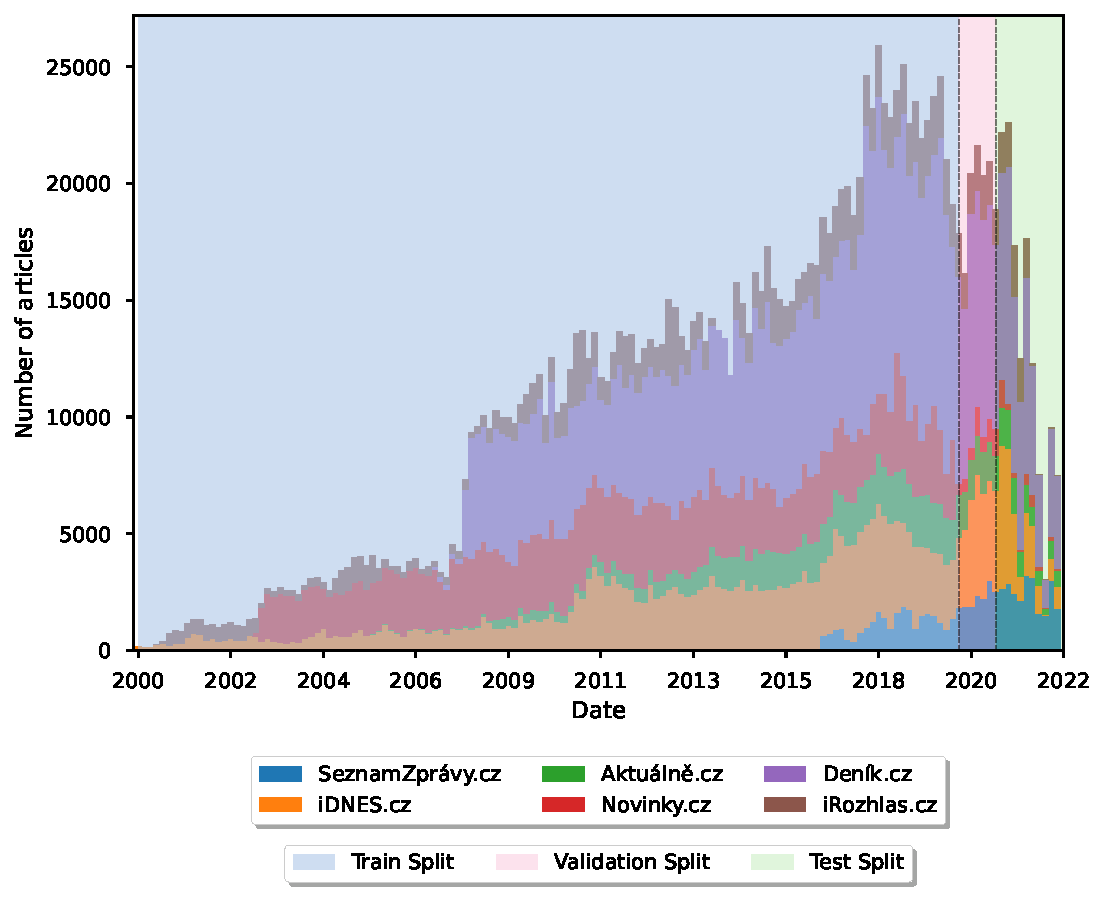
\includegraphics[width=1.0\textwidth]{img/dataset_evolution/evolution.pdf}
    \caption{Distribution of news servers over time with dataset split boundaries.}
    \label{fig:evolution}
\end{figure}
We divided the dataset into the train, validation, and test sets based on
publication date, using a 34:3:3 ratio. The sets are ordered by publication date, i.e., the train set contains the earliest articles, while the test set contains the latest articles.
The dataset division is depicted in \autoref{fig:evolution}.

Due to experiments, we also additionally created the following splits:
\begin{enumerate}
    \item\label{enum:train-small} \textbf{Train Small} - 50K most recent samples from the training set, containing all metadata
    \item\label{enum:test-small} \textbf{Test Small} - 10K randomly selected samples from the test set, containing all metadata
    \item\label{enum:test-human} \textbf{Test Human} - 100 randomly selected samples from the test set, containing all metadata
\end{enumerate}

\section{Dataset Summary}
\begin{table}[t]
    \resizebox{\linewidth}{!}{%
        \caption{Dataset summary. Article words were calculated based
            on Moses tokenization.}
        \label{tab:dataset_summary}
        \centering
        \begin{tabular}{lrrrrr}
            \toprule
            Server          & Size    & Authors & Categories & Start date            & Words per article \\
            \midrule
            Deník.cz   & \hphantom{1,}664,133  & \hphantom{1}2,497           & 18         & 2007  & 332           \\
            Novinky.cz   & \hphantom{1,}321,417  & \hphantom{1}2,518           & 17         & 2002 & 274           \\
            iDnes.cz & \hphantom{1,}295,840  & \hphantom{1}4,386           & 21         & 2000   & 423           \\
            iRozhlas.cz   & \hphantom{1,}167,588  & \hphantom{1}1,900           & 8          & 2000  & 287           \\
            Aktuálně.cz   & \hphantom{1,}112,960  & \hphantom{10,}633            & 19         & 2005 & 468           \\
            SeznamZprávy.cz~~~ & \hphantom{1,0}65,472   & \hphantom{10,}382            & 11         & 2016  & 443           \\
            \midrule
            Total       & 1,627,410 & 10,930          & 25         & 2000   & 362           \\
            \bottomrule
            \\
        \end{tabular}
    }
\end{table}
The summarization of the dataset is shown in~\autoref{tab:dataset_summary}.
The dataset contains the following features:
\begin{itemize}
    \item \emph{Server} - Server that published the article
    \item \emph{Content} - Actual text content of the article
    \item \emph{Brief} - Brief/Perex of the article
    \item \emph{Headline} - Headline/Title of the article
    \item \emph{Category} - Both post-processed and original category
    \item \emph{Published Date} - Date of publication and inferred day of week
    \item \emph{Authors} - List of article authors
    \item \emph{Inferred gender} - Inferred gender of author(s) name(s)
    \item \emph{Keywords} - Extracted keywords from the article
    \item \emph{Comments Count} - Number of comments in the discussion section
\end{itemize}

\section{Task Definitions}\label{sec:task_definition}
\begin{table}[h]
        \caption{Tasks distribution over sets.}
        \label{tab:task_distribution}
        \centering
        \begin{tabular}{lrrrr}
        \toprule
        Set &   Server &  Category &  Gender &  Day of week \\
        \midrule
        Train      &  1,383,298 &             \hphantom{1,}879,019 & \hphantom{1,}919,840 &      1,383,298 \\
        Validation &  \hphantom{1,}122,056 &  \hphantom{1,0}78,084 & \hphantom{1,0}82,936 & \hphantom{1,}122,056 \\
        Test       &  \hphantom{1,}122,056 &  \hphantom{1,0}82,352 & \hphantom{1,0}83,269 & \hphantom{1,}122,056 \\
        \midrule
        Total   &   1,627,410 &  1,039,455 &           1,086,045 &    1,627,410  \\
        \bottomrule
        \end{tabular}
\end{table}
We provide more details about the tasks in this section.
Each task is provided an article body as input, excluding the brief and headline.
As not all metadata are available for all articles, we show the distribution of samples over sets
in~\autoref{tab:task_distribution}.


\subsection{Server}
\label{sec:server-desc}
\begin{figure}[ht]
    \centering
    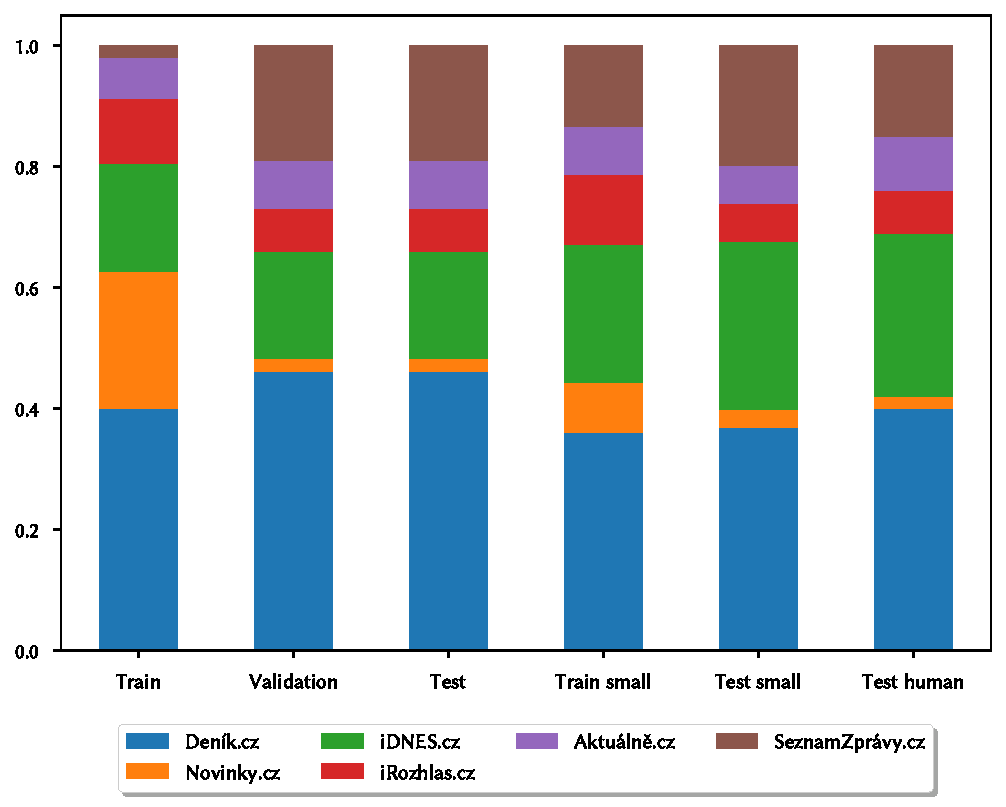
\includegraphics[width=1.0\textwidth]{img/tasks_graph/server.pdf}
    \caption{Graph depicting proportion of servers among the datasets.}
    \label{fig:server_graph}
\end{figure}
The Server classification task involves predicting the publishing server
of articles from a set of 6 labels, as shown in~\autoref{fig:server_graph}. It is important to note
that there is a significant distribution shift between the training and validation
set, which is caused by differences in the launch dates of the servers and parsing
issues (especially with Novinky.cz)


\subsection{Category}
\begin{figure}[ht]
    \centering
    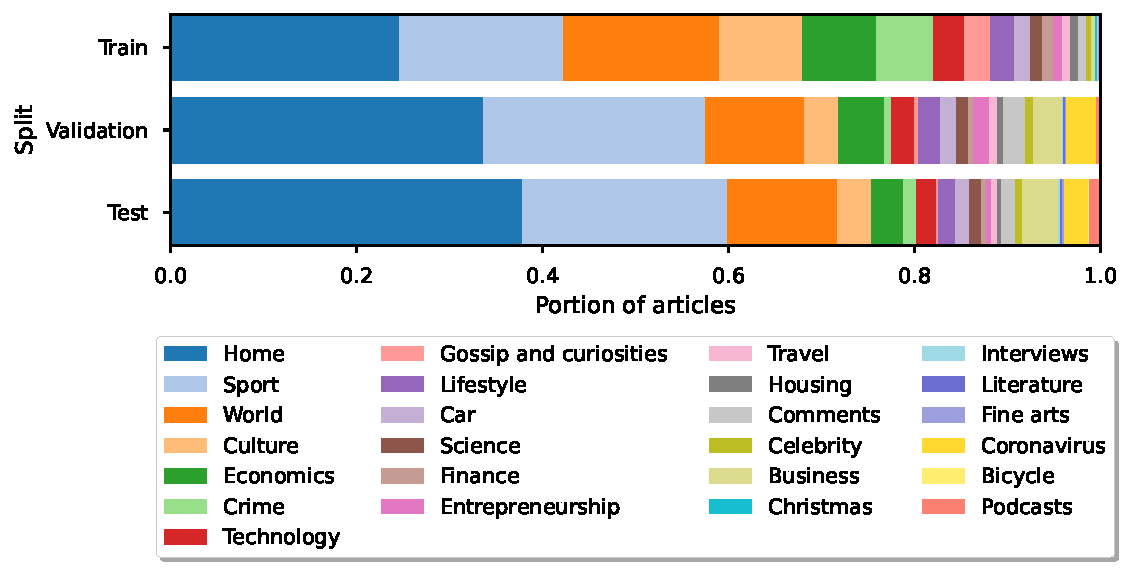
\includegraphics[width=1.0\textwidth]{img/tasks_graph/category.pdf}
    \caption{Graph depicting distribution categories among the datasets.}
    \label{fig:category_graph}
\end{figure}
The Category classification task requires predicting the category of
an article from a set of 25 labels, as depicted in~\autoref{fig:category_graph}. When selecting the
categories, we carefully identify the most frequent ones while striving to maintain
diversity and minimize any potential overlap between them.

\subsection{Gender}
\begin{figure}[h]
    \centering
    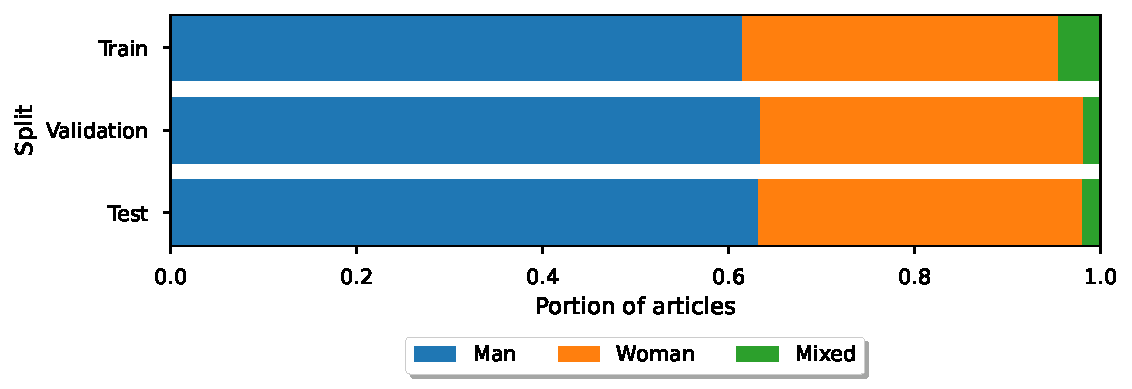
\includegraphics[width=1.0\textwidth]{img/tasks_graph/authors_cum_gender.pdf}
    \caption{Graph depicting the distribution of genders among the datasets.}
    \label{fig:gender_graph}
\end{figure}
This classification task has 3 labels, as shown in~\autoref{fig:gender_graph}.
Its goal is to predict the inferred gender of the article author(s). While we are aware
that the inferred gender is not always correct, we think that it serves as a good proxy predicted, due to the strong
association of social and grammatical gender in the Czech language.
This task is not meant to label individuals and the text they produce, and we discourage future users of CZE-NEC from doing so.

\subsection{Day of the Week}
\begin{figure}[h]
    \centering
    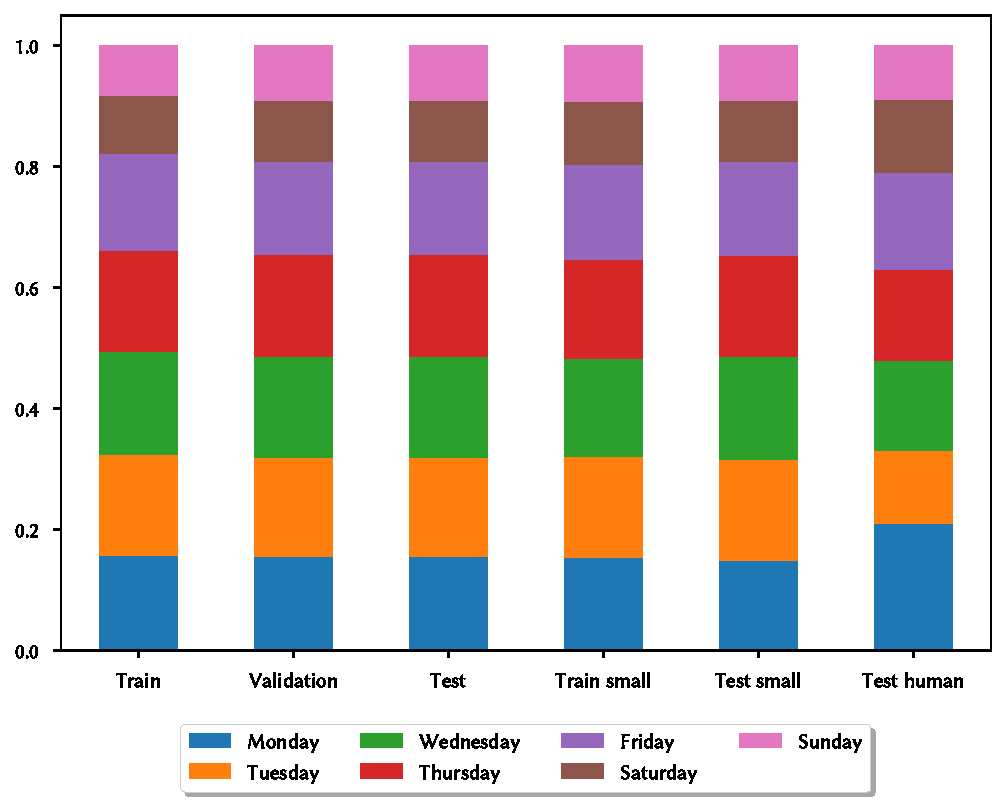
\includegraphics[width=1.0\textwidth]{img/tasks_graph/day_of_week.pdf}
    \caption{Graph depicting the distribution of weekdays among the datasets.}
    \label{fig:day_graph}
\end{figure}
The Day of Week task is a classification challenge consisting of seven distinct labels, as illustrated in~\autoref{fig:day_graph}.
The objective is to
accurately predict the day of the week a given article was published. Given the
absence of any apparent approaches to tackle this task, we deem it to be the
most challenging among the tasks considered.